%!TEX root = ../Master.tex

\section{Hardware} % (fold)
\label{sec:hardware}

As mentioned in \autoref{sec:prokect_introduction} the focus of the project have been on the software implementations of theory learned throughout the course. By using a Neato XV-11 vacuum cleaning robot in \autoref{fig:neato_xv11} which have a build-in lidar to sense its environment, and that implements functionality to move by some unit distance, most hardware concerns have been eliminated.\\

\begin{figure}[H]
\centering
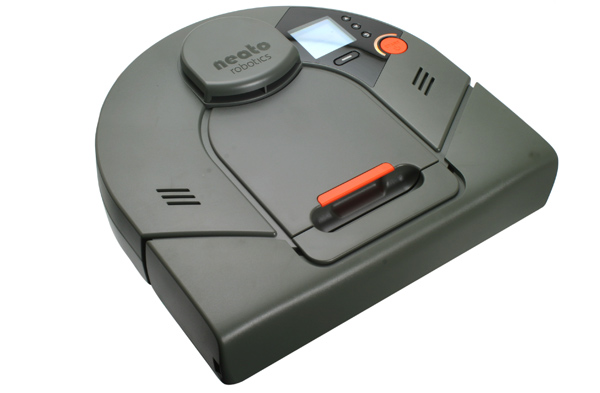
\includegraphics[scale=0.40]{images/neato_xv11}
\caption{Neato XV-11}
\label{fig:neato_xv11}
\end{figure}

The lidar is also developed by Neato and ...\\
\fxnote{Add facts about lidar, and maybe other things about the robot hardware.}

The Neato robot runs ROS which makes it possible to develop and simulate the robot on a PC, and the code can then to loaded onto the robot and executed.\\
However, there are some discrepancies between simulation and real-life execution regarding lidar measurements, which have hindered testing on the actual robot.

% section hardware (end)